% !TEX root = ~/OpenFOAM/antoniopucciarelli-9/run/LABS/thermochemical_CFD/main.tex

\section{Lagrangian particles tracking and wall-film modeling - $\mathtt{Lab05}$ and $\mathtt{Lab06}$}
    
    \renewcommand{\thepage}{\arabic{page}}
    \setcounter{page}{\thelastPage}
Spray modeling and wall-film theory are described in appendix~\ref{app:app3_1} and appendix~\ref{app:app3_2}.    
%    \subsection{Spray modeling}
%    \subsubsection{Spray description and lagrangian particles approach}
%    Sprays are largely used in the combustion field. The aim is to let the fuel evaporate in the shortest time possible to reach the best performances.
%    Engineers have divided the spray in 3 regions and one of the main describers can be the void fraction\footnote{$\alpha = \frac{V_{liquid}}{V_{cell}}$}: 
%    \begin{itemize}
%        \item \textbf{Dense region} In this region, there is the first break up of the jet core in many string shaped drops. The fuel has a low surface to volume ratio, this implies the fuel is a dense and confined region in the system. This region has to be treated with care and it is very computationally demanding. The models required to solve this region are called \textbf{continuous phase models}, \verb|CPM|. The void fraction for this region is around unity. 
       
%        \item \textbf{Diluted region} In this region, the dense region starts to break up into smaller pieces; these pieces have a larger surface to volume ratio but not high enough to be modelled as spheric particles. This region is very important to lagrangian particles tracking methods because it is the region of transition between dense to dispersed region. This region can be treated as well with \verb|CPM|. The final aim of the \verb|CPM| in this case is to get a good description of the spray properties for the dispersed region modeling. The void fraction is around $0.5$ - this because $\frac{V_{liquid}}{V_{gas}} \approx 1$.
        
%        \item \textbf{Dispersed region} This region consists of many dispersed particles where the surface to volume ratio is high enough to consider these particles as spheres. This \textbf{huge} simplification allows using the lagragian spray method for the modeling of the development of the spray in the dispersed region\cprotect\footnote{It is possible to model the dispersed region with \verb|CPM|. Using \verb|CPM| in the dispersed region means not considering the particles as spheres. \verb|CPM| in dispersed region is very computational demanding and very difficult to handle.}. In the following CFD cases, lagrangian particles models are used to discretize the spray evolution (dispersed region only) into the system. As result of dispersed fuel into the system, the void fraction is lower than $1$.
%    \end{itemize}

%    \subsubsection{Parcels in spray modeling}
%    The number of particles in the dispersed region can be of order of billions; this will bring a lot of computational effort to model all the particles into the system and also to store all the data related to particles' properties, position and dynamics. In order to solve this problem, lagrangian sprays adopted a new way of modeling for these particles.
%    All these particles are grouped into objects called parcels. The grouping process is related to the particles' diameter. If a particle has a certain diameter, this particle will be grouped with other particles that fall inside a defined diameter range. Particles' diameter is defined by experimental results, by results analysis of dense and diluted region simulations and by statistics. After the grouping process, every parcel in the system has defined properties. The lagrangian spray modeling will compute the parcels evolution into the system. 
    
%    \paragraph{Parcels interaction}
%    Since parcels represent the properties of group of particles, the evolution of parcels represents the evolution of those particles. Parcels and gaseous flow can interact in different ways. This depends on the nature of the spray, on parcels' properties and on computational power available. It is possible to model the spray as:
%    \begin{itemize}
%        \item \textbf{One way coupling} The one way coupling allows only a \textit{one way talk} from the continous phase to the discrete phase. This allows to compute the parcels motion directly from the continuous phase field. Of course, parcel motion depends on the forces applied to it; these forces are computed using forces equations applied to spherical shaped particels with the help of experimental results. The forces' models depend on particles diameter - expressed through parcel object -, the particles diameter on the other hand depends on the thermodynamics (because of evaporation).
%        \item \textbf{Two ways coupling} The two way coupling allows the \textit{talk back} of the discrete phase evolution to the continous phase. This happens through additional source terms in the continuous phase equations. As result, this method is more computational demanding\footnote{All the modeling aspects for the parcel's evolution are the same as the one way coupling}.
%        \item \textbf{Four ways coupling} The four ways coupling accounts also to the parcels interaction. Usually this method is used when $\alpha \geq 10^{-2}$. The continuous phase treatment remains almost the same as the two ways coupling but the parcels interaction has an additional modeling step that takes into account the changes parcels make into the continuous field because their distance and also the parcels interaction as parcels agglomeration and parcels break-up.
%    \end{itemize}

%    \subsection{Wall-film modeling}
%    The particles-wall interaction has to be treated by the simulation. This interaction is very important because it can change a lot the behaviour of the solution. Wall-film in OpenFOAM are mainly treated using these hypothesis:
%    \begin{itemize}
%        \item \textbf{Wall-film thickness hypthesis} The wall-will thickness is supposed to be very thin; this brings to study the liquid film evolution as a 2D problem
%        \item \textbf{Particles temperature change} The temperature change of the particles impinging the wall-film is slow; this allows direct analytical time integration istead of numerical integration
%        \item \textbf{Conductivity hypothesis} Since the wall-film region is a layer above the solid wall, heat is transmitted from the wall to the liquid film through conductive mechanism
%        \item \textbf{Temperature limits hypothesis} Due to modeling reasons, the wall and wall-film temerature is supposed to be lower than the liquid boiling temperature
%    \end{itemize}
%
%    \subsubsection{Mesh and boundary conditions}
%    Because the wall-film region can be seen as an additional model to the usual \verb|FVM| case, a mesh has to be built in order to study the wall-film region. The only purpose of the wall-film mesh is to track the development of a 3D wall-film using a 2D mesh. The wall-film has to talk back to the \textit{global} mesh in order to set up correct boundary conditions for the main flow. As result of this modeling choices, the main parameters that describe the wall-film region are:
%    \begin{itemize}
%        \item $\delta$ Liquid film height. Since the mesh is 2D, the wall film height is described by $\delta$ but at the same time $\delta$ describes the presence of the liquid film on the wall-film region surface
%        \item $\boldsymbol{u}$ Liquid film velocity
%        \item $T$ Liquid film temperature
%    \end{itemize}
%    
%    Transport equations~(\ref{eqn:transp}) are used for tracking these quantities:
%    \begin{equation}
%        \begin{cases}
%            \frac{\partial \rho \delta}{\partial t}  + \boldsymbol{\nabla} \cdot \big( \rho \ \delta \ \boldsymbol{u} \big) & = \boldsymbol{S}_{\delta} \\ 
%            \frac{\partial \rho \delta \boldsymbol{u} }{\partial t}  + \boldsymbol{\nabla} \cdot \big( \rho \ \delta \boldsymbol{u} \ \boldsymbol{u} \big) & = \boldsymbol{S}_{\delta \boldsymbol{u}} \\ 
%            \frac{\partial \rho \delta h }{\partial t}  + \boldsymbol{\nabla} \cdot \big( \rho \ \delta h \ \boldsymbol{u} \big) & = \boldsymbol{S}_{\delta h}
%        \end{cases} \label{eqn:transp}
%    \end{equation}

    \subsection{Problem setup}
    It is possible to see this new case as the previous compressible case plus two \textbf{additional layers} of modeling: the lagrangian particles evolution and the surface wall-film modeling. 
    These new layers are described by defined dictionaries. The \verb|fvModels| allows to enable these dictionaries and to \textbf{wrap} them into the \textit{main} case. The wall-film region is generated through the \verb|topoSet| dictionary. This dictionary coverts patch of the system into \verb|faceSet| or \verb|faceZoneSet| objects; these objects allow to make new operations such as wall-film region generation. The wall-film region is made using the \verb|extrudeToRegionMesh| dictionary. This dictionary makes a one layer 2D mesh from the patch converted by \verb|topoSet| firstly into \verb|faceSet| and then into \verb|faceZoneSet|. As additional step, it is necessary to change the boundary conditions; this means that the \textit{main} field and the wall-film region field (in \verb|0/wallFilmRegion|) have to set their boundary conditions on the \verb|faceZoneSet| generated\cprotect\footnote{This is done through the \verb|bash| script \verb|AllSplitterRegion|.}. 

    \cprotect\subsubsection{\verb|cloudProperties|}
    This dictionary is a describer of the injector properties. The injector properties are summed up in parcels number, velocity, temperature, distribution and timing. These properties are assigned in \verb|subModels -> injectionModels|. The force applied to the parcels are described in \verb|particleForces|; only drag forces are present. The distribution model used is the \verb|RosinRammler|. The interaction between parcel and wall is set as \verb|rebound| (particle bumps on the surface). Particles diameter is allowed to change with an evaporation model set as \verb|liquidEvaporationBoil|\cprotect\footnote{Every chemical property of the liquid is described in \verb|chemkin| folder and converted into OpenFOAM syntax with \verb|chemkinToFoam| command in \verb|bash|.}. \verb|breakupModel| describes the particle break up interaction into the simulation.   

    \cprotect\subsubsection{\verb|surfaceFilmProperties|}
    The liquid film modeling is described by a complicated dictionary that containts in itself many submodels. These submodels are describers of the interaction of the wall-film with the \textit{main} flow. \verb|viscosity|, \verb|momentumTransport|, \verb|forces| and \verb|ejection| are the main subdictionaries. The \verb|ejection| subdictionary describes the interaction of the liquid film with the splitter geometry with respect to its \textbf{shape}. 
    
    \subsection{Post-processing}
    The post-processing setup is different from the previous cases. There exist different ways to get the results. Using the python code \verb|latexData.py|, data from parcels size distribution and liquid penetration are available. A useful post-processing tool is \verb|foamToVTK|. This command allows to reconstruct the case and all its properties in \verb|VTK| format.

    \subsection{Result}
    The main differences between the different cases consist into particles breakup model - in \verb|cloudProperties| - and \textit{main} flow temperature. 
    
    \cprotect\subsubsection{\verb|combustorSprayWallFilmReitzKHRT|}
    This case uses the \verb|ReitzKHRT| breakup model. The effect of \verb|rebound| setting in \verb|cloudProperties| is very evident in the final solution. The particle jet reaches its maximum amplitude at the middle of the simulation due the the \verb|sine| flow rate setting. Most of the particles impinges on the splitter. There are particles that are still not fully evaporated after passed the splitter. 

    \cprotect\subsubsection{\verb|combustorSprayWallFilmReitzDiwakar|}
    This case uses the \verb|ReitzDiwakar| breakup model. The jet behaviour is similar to the \verb|ReitzKHRT|. There are changes in the particles distribution over time and of the liquid penetration. The reason relies in the way the breakup of the parcels is modeled; it is like the \verb|ReitzDiwakar| treats the particles as less interactive with the environment (this explains why the liquid jet penetration is a bit higher than \verb|ReitzKHRT|).

    \cprotect\subsubsection{\verb|combustorSprayWallFilmReitzKHRT450|}
    This last case uses the \verb|ReitzKHRT| breakup model and \verb|fixedValue -> value 450;| as boundary condition for the \verb|T| at the \verb|inlet|\cprotect\footnote{The other two cases used \verb|fixedValue -> value 300;| as inlet temperature boundary condition.}. The solution is completelly different from the previous ones. This because the higher temperature of the \textit{main} flow that allows faster evaporation of the parcels into the system.

    \newpage

    % PAGE MANAGEMENT 
    \setcounter{lastPage}{\thepage}
    \renewcommand{\thepage}{SWF-\roman{page}}
    \setcounter{page}{1}

    \begin{figure}[!ht]
        \centering
        \import{latexFIGS/lab0506/}{residuals.pgf}
        \caption{Surface \& wall-film cases: residuals.}
    \end{figure}

    \begin{figure}[!ht]
        \centering
        \import{latexFIGS/lab0506/}{phase95.pgf}
        \caption{Surface \& wall-film cases: liquid penetration.}
    \end{figure}

    \begin{figure}[!ht]
        \centering
        \import{latexFIGS/lab0506/}{diam.pgf}
        \caption{Surface \& wall-film cases: parcels diameter.}
    \end{figure}

    \begin{figure}[!ht]
        \centering
        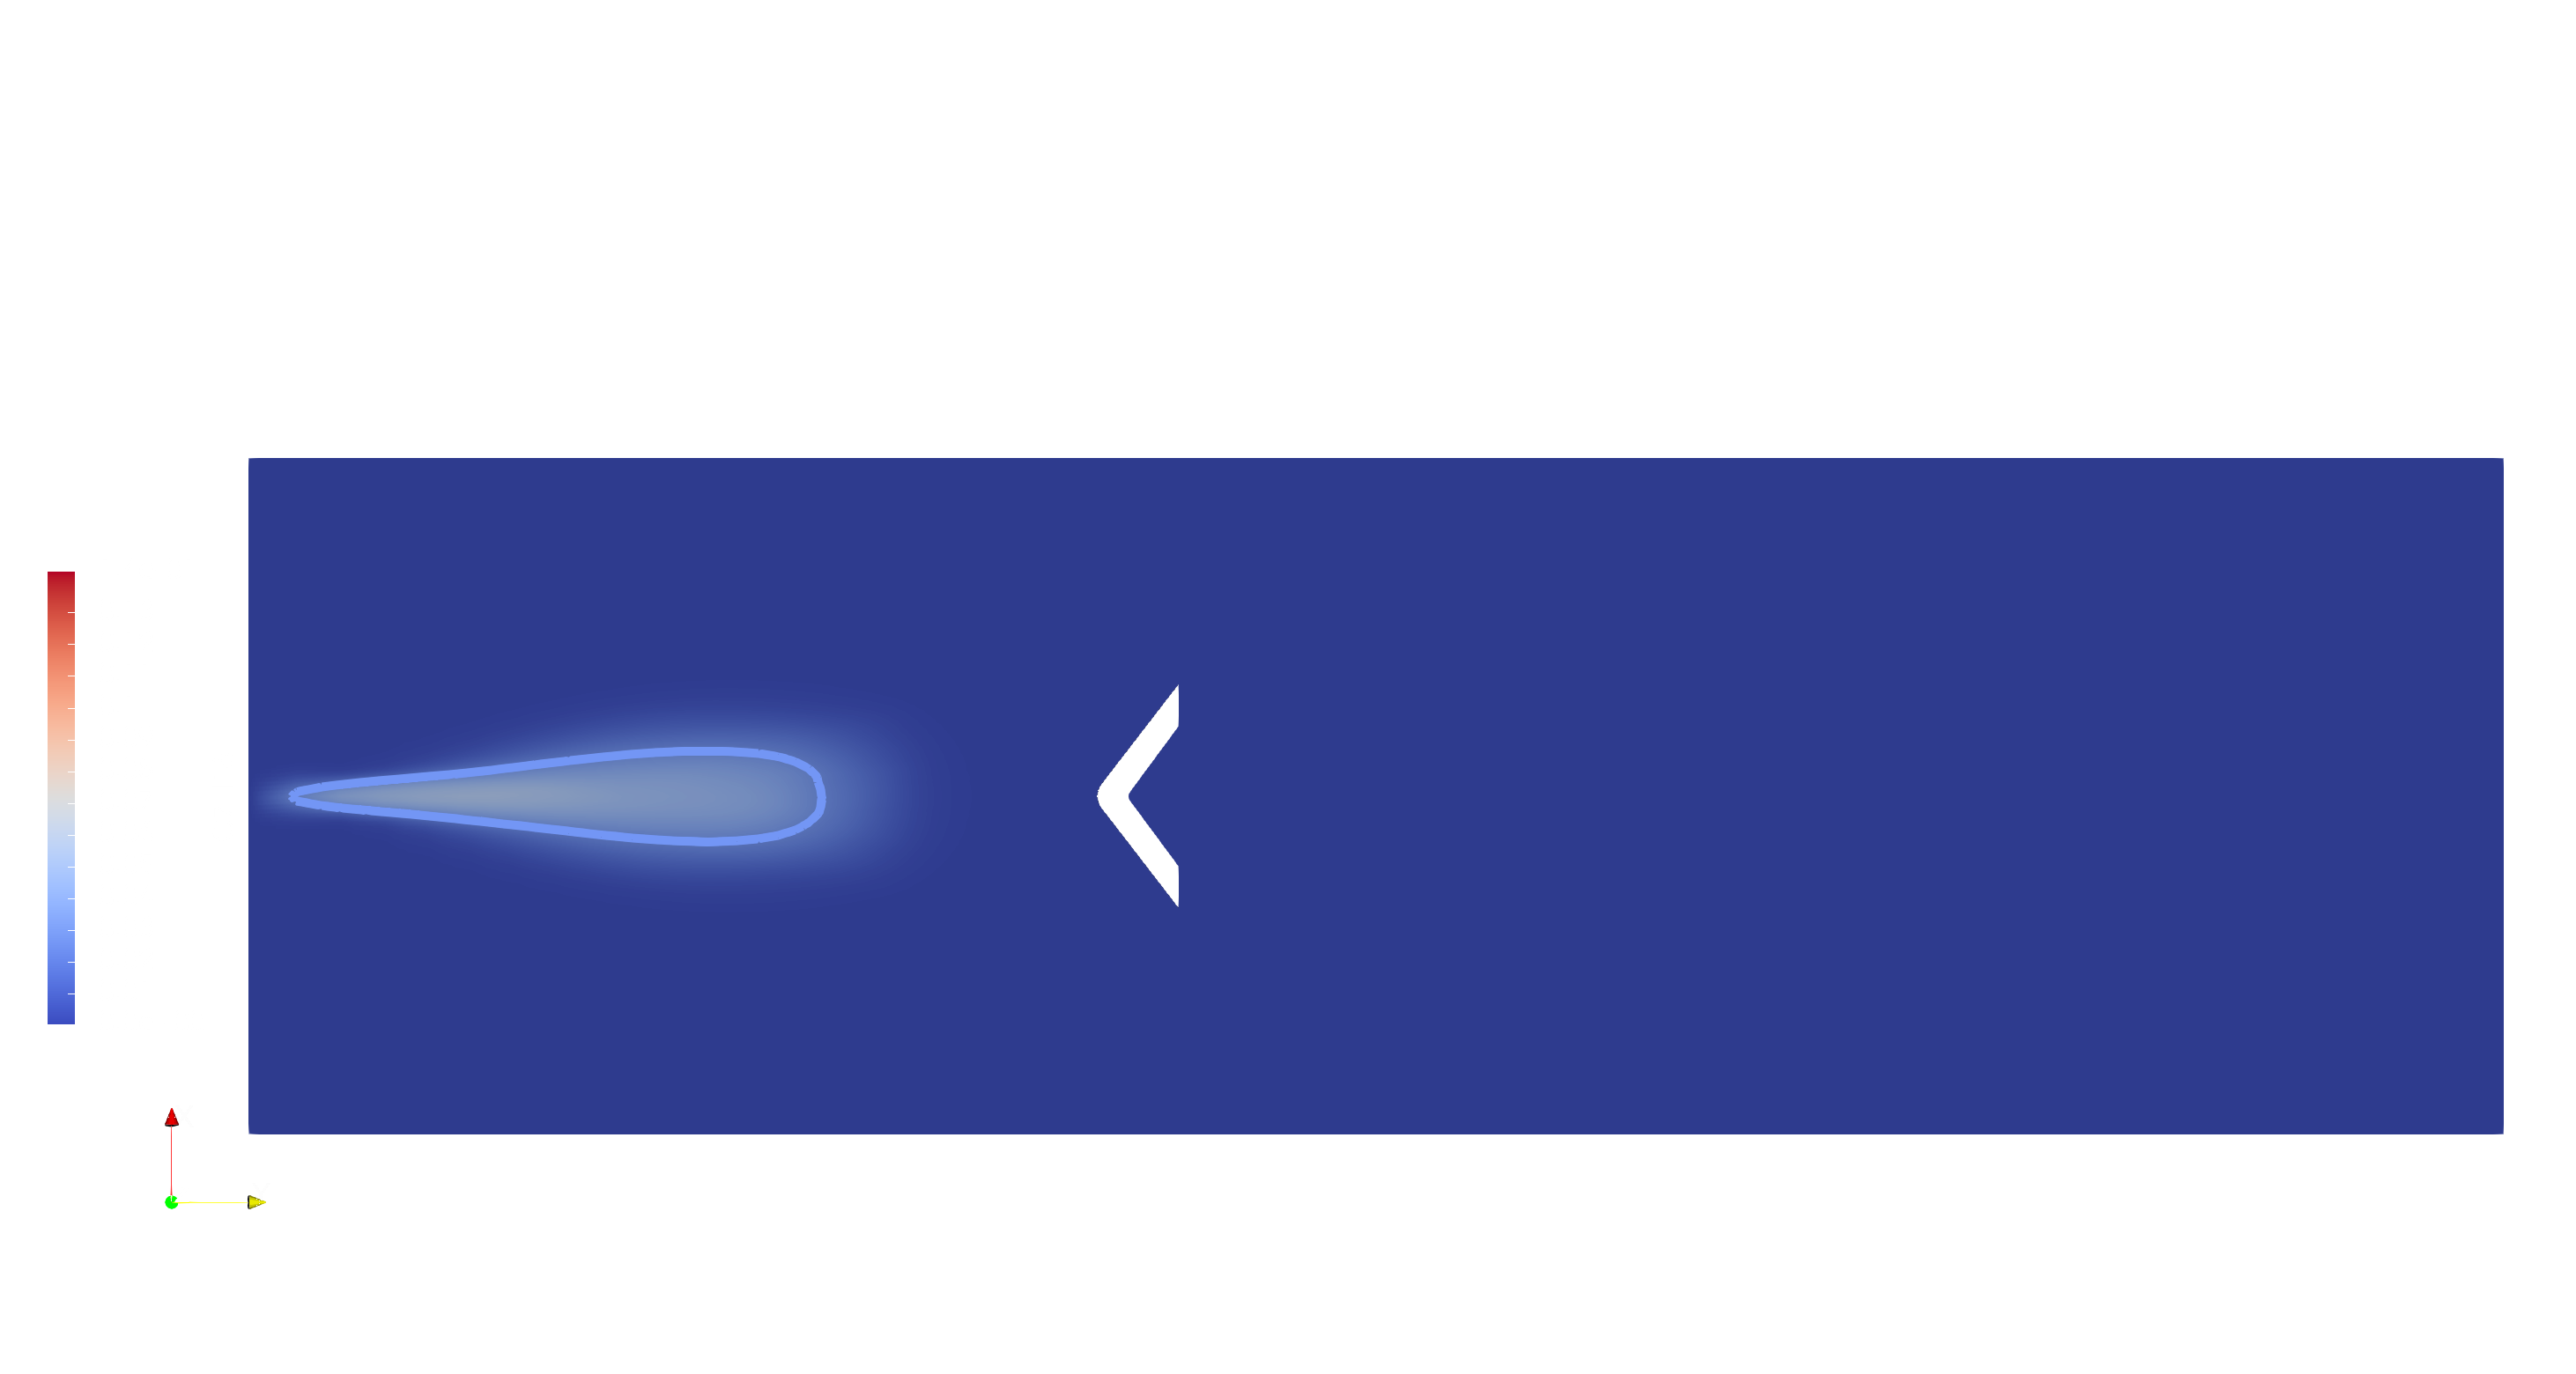
\includegraphics[height=0.25\textheight]{latexFIGS/figs/combustorC7H16_002.png}
        \cprotect\caption[\verb|C7H16| evaporation contour tracking, $t = 0.02s$.]{\verb|C7H16| evaporation contour tracking, $t = 0.02s$. \\ \verb|combustorSprayWallFilmReitzDiwakar|}
    \end{figure}
    
    \begin{figure}[!h]
        \centering
        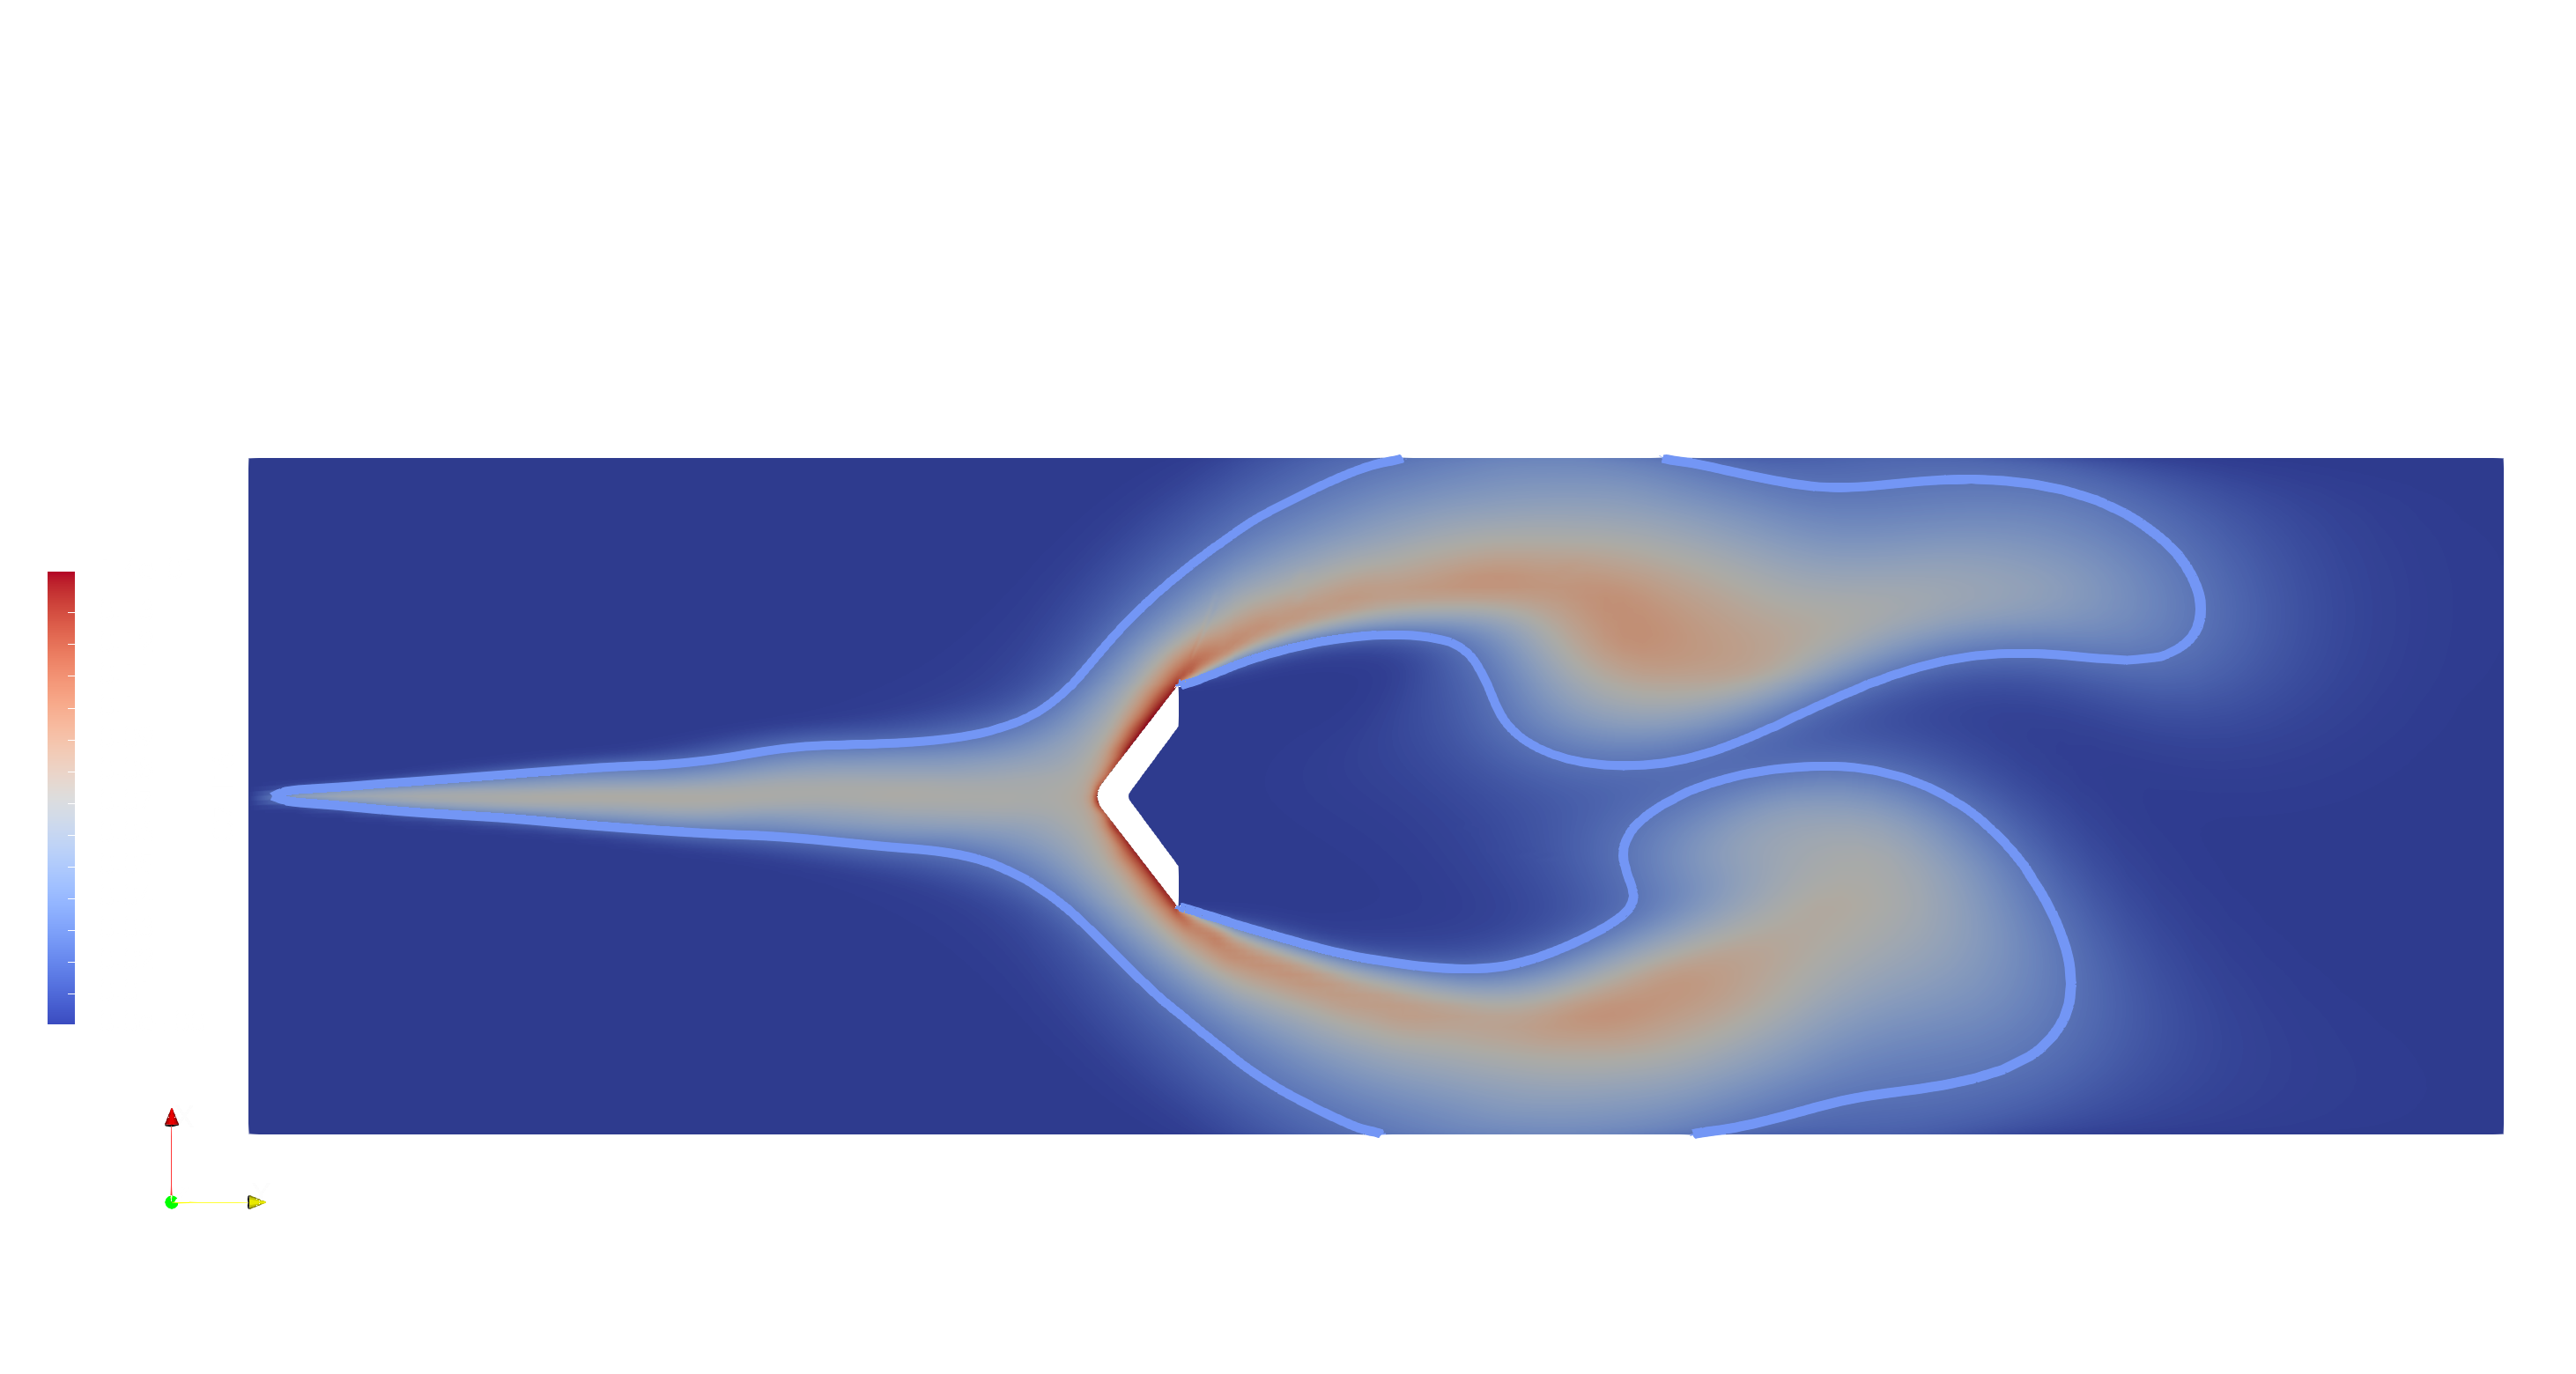
\includegraphics[height=0.25\textheight]{latexFIGS/figs/combustorC7H16_005.png}
        \cprotect\caption[\verb|C7H16| evaporation contour tracking, $t = 0.05s$.]{\verb|C7H16| evaporation contour tracking, $t = 0.05s$. \\ \verb|combustorSprayWallFilmReitzDiwakar|}
    \end{figure}
    
    \begin{figure}[!hb]
        \centering
        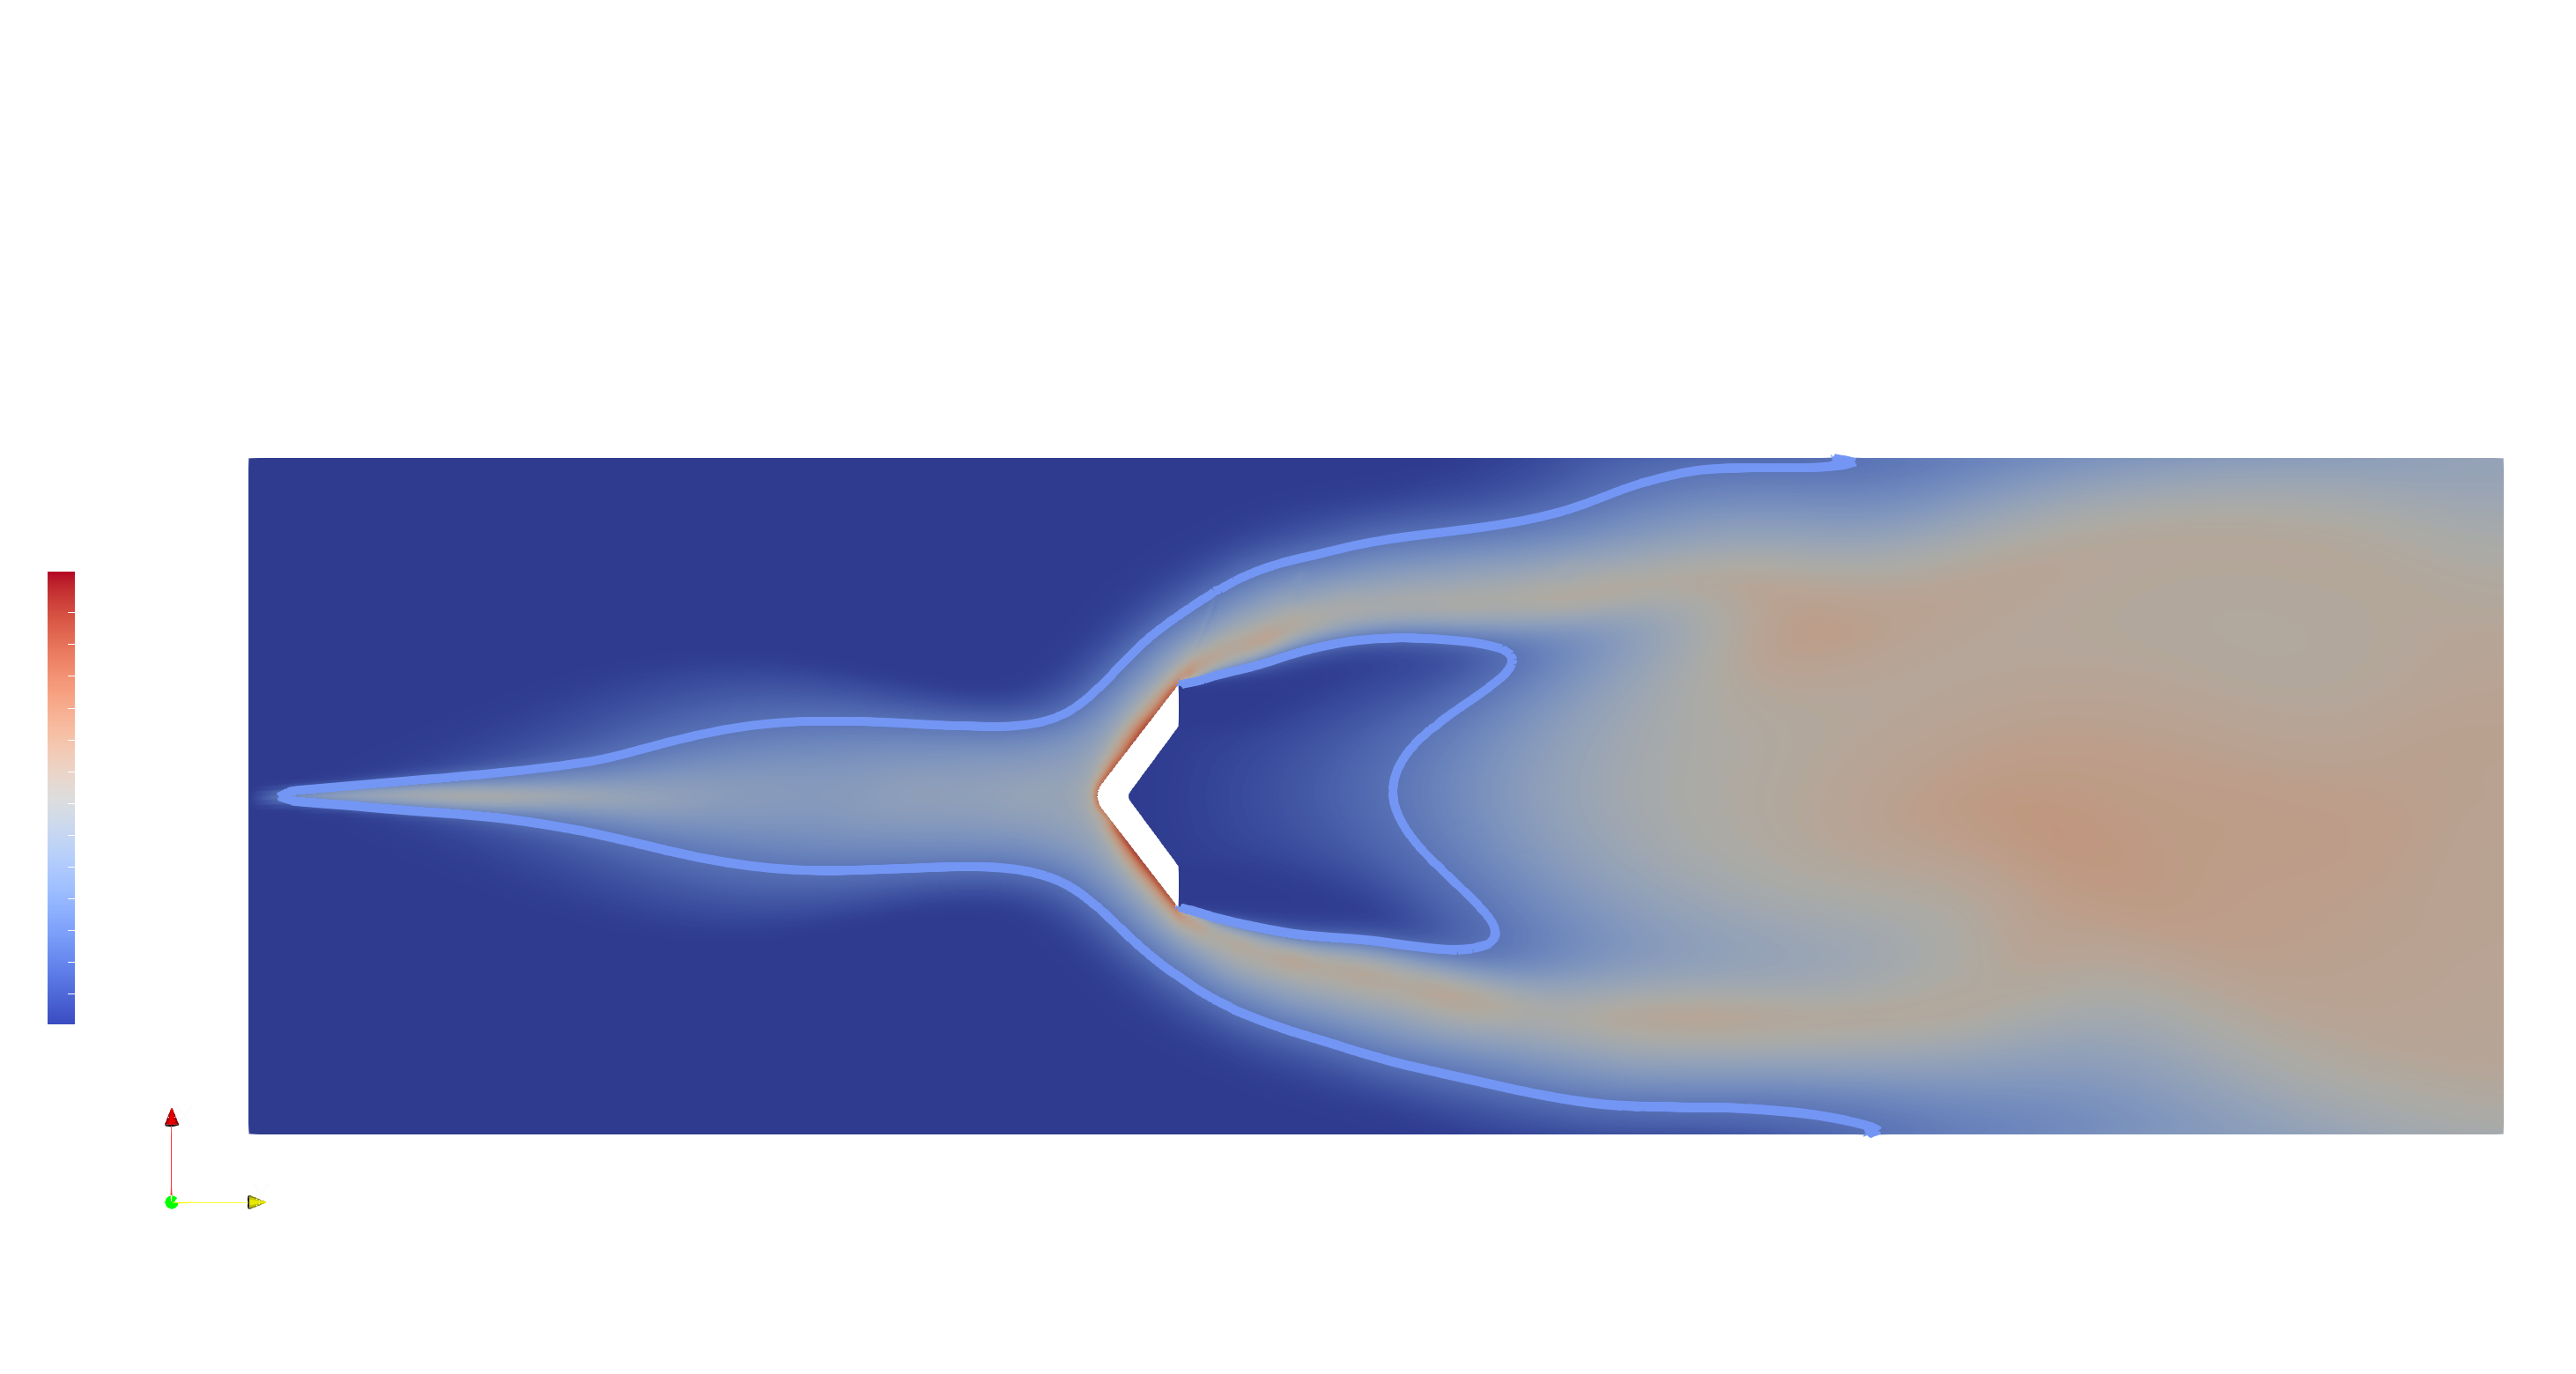
\includegraphics[height=0.25\textheight]{latexFIGS/figs/combustorC7H16_008.png}
        \cprotect\caption[\verb|C7H16| evaporation contour tracking, $t = 0.08s$.]{\verb|C7H16| evaporation contour tracking, $t = 0.08s$. \\ \verb|combustorSprayWallFilmReitzDiwakar|}
    \end{figure}

    \clearpage
